\documentclass[addpoints]{exam}
\pagestyle{headandfoot}
\firstpageheadrule
\runningheadrule
\firstpageheader{CT - Topic 1}{}{Sam Robbins}
\runningheader{CT - All}{}{Sam Robbins}
\firstpagefooter{}{}{}
\runningfooter{}{}{}
\renewcommand{\solutiontitle}{\noindent\textbf{Solution:}\par\noindent}

\usepackage{listings}
\usepackage{amsmath}
\usepackage{amssymb}
\printanswers
\usepackage{graphicx}
\marksnotpoints
\bracketedpoints
\pointsdroppedatright
\pointsinrightmargin
\lstset{language=Python,
	basicstyle=\ttfamily,
	keywordstyle=\bfseries,
	showstringspaces=false,
	morekeywords={if, else, then, print, end, for, do, while,output},
	tabsize=4,
	mathescape=true,
	moredelim=**[is][\color{red}]{@}{@},
}
\begin{document}
\begin{center}
	\underline{\huge Questions likely to be on the exam}
\end{center}
\begin{questions}
\question[1]What are the two main components of an integrated circuit? (Both of
these components usually appear in their millions.)
\begin{solution}[2in]
	Transistors [$\frac{1}{2}$] interconnected by microscopic wires [$\frac{1}{2}$].
\end{solution}


\question[2]What is the current trend in microprocessor design so as to overcome
difficulties with power dissipation as we build faster and faster single
processors?
\begin{solution}[2in]
	Multi-core processors [1] where one CPU with a high clock-speed is
	replaced with a number of CPUs with lower clock-speeds but which,
	when working together, can give better computational power [1].
\end{solution}
\question[10] What is a NAND-gate? Show how a NOT-gate, an AND-gate and an
OR-gate can be constructed using just NAND-gates
\begin{solution}[2in]
	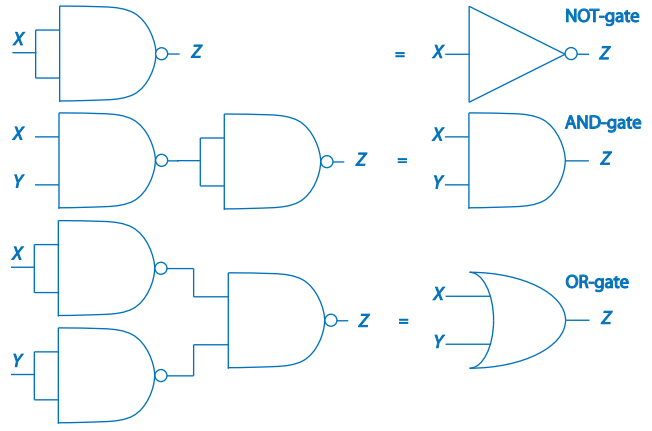
\includegraphics[width=8cm]{NAND.png}
\end{solution}


\question[7]What are a half-adder and a full-adder? Show how a full-adder can be
built using 2 half-adders
\begin{solution}[2in]
	A half-adder takes x and y as inputs and computes the Boolean sum
	of x and y, where the Boolean sum of a collection of inputs is 1 if, and
	only if, an odd number of the inputs are 1, and also the resulting carry
	bit, which is 1 if, and only if, both x and y are 1 [2]. A full-adder takes
	x, y, and z as inputs and computes the Boolean sum of x, y, and z,
	resulting in the sum-bit and the carry-bit [2].\\
	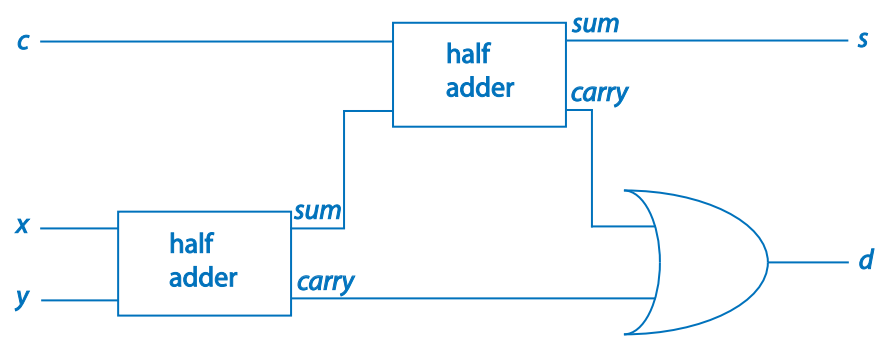
\includegraphics[width=8cm]{full_adder.png}
\end{solution}

\begin{solution}[2in]
	The von Neumann bottleneck is a limitation of the rate of data transfer
	between the CPU and memory (data and instructions have to be
	fetched in sequential order and idle time is wasted whilst waiting for
	data items or instructions to be fetched from memory) [2]. The von
	Neumann bottleneck gave rise to the use of caches [1].
\end{solution}


\question[2]How does the Harvard architecture differ from the von Neumann architecture?
\begin{solution}[2in]
	The Harvard architecture has memory that is partitioned into data
	memory and instruction memory with dedicated buses for each of them
	[2].
\end{solution}

\question[6]Name two types of bus within a CPU and explain the general purpose
of each. What is the width of a bus? Explain how the width of a bus
imposes memory or data limitations within a CPU.
\begin{solution}[2in]
	Buses include a \textbf{data bus} $[\frac{1}{2}]$, an \textbf{address bus} $[\frac{1}{2}]$ and a \textbf{control bus} $[\frac{1}{2}]$. A data bus carries the contents of memory locations between the
	processor and main memory $[\frac{1}{2}]$. The address bus holds addresses of
	locations in main memory $[\frac{1}{2}]$. The control bus is used to transfer
	information between the CPU and various other devices within the
	processor $[\frac{1}{2}]$. The width of a bus is the number of parallel wires in
	a bus [1]. The width of the data bus determines the word-size of the
	computer [1]. The width of an address bus determines the size of
	addressable memory [1].
\end{solution}

\question[3]What is the difference between static RAM and dynamic RAM?
\begin{solution}[2in]
	Dynamic RAM (DRAM) is where a bit of data is stored using a transistor/capacitor
	combination [1]. Static RAM (SRAM) is where a bit
	of data is stored by a flip-flop, which incorporates 4-6 transistors [1].
	Static RAM is stable and fast but takes up more memory $[\frac{1}{2}]$ whereas
	dynamic RAM is cheap, slow and needs to be refreshed because of
	‘leaky’ capacitors $[\frac{1}{2}]$.
\end{solution}


\question[1]What is the purpose of cache memory in a CPU?
\begin{solution}[2in]
	Caches are expensive memory that are used to store rapidly accessed
	items [1].
\end{solution}

\question[5]Explain carefully the four phases of the fetch-decode-fetch-execute processor cycle (be sure to explain the purpose of any CPU components
you happen to mention).
\begin{solution}[2in]
	The ‘\textbf{instruction fetch}’ phase involves the supply of the instruction address
	(via the address bus) and the return from memory (via the data
	bus) of the instruction [1]. The ‘\textbf{instruction decode}’ phase involves
	interpreting the stored instruction within the CPU [1]. The ‘\textbf{operand
		fetch}’ phase involves the supply of the address of any required data (via
	the address bus) and the return from memory (via the data bus) of this
	data [1]. The ‘\textbf{execute instruction}’ phase involves the CPU performing
	the necessary actions [1] (this phase is sometimes split into two with
	the ‘execute instruction’ phase followed by a ‘write-back’ phase where
	data is written back to memory, if needs be [1]).
\end{solution}

\question[4]Show different layers of abstraction in a modern computer system.
\begin{solution}[2in]
	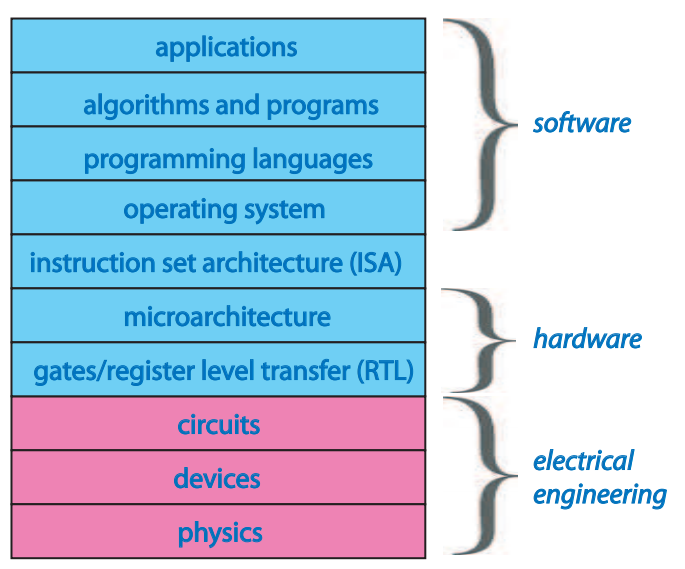
\includegraphics[width=8cm]{CSys.png}
\end{solution}

\question[5]Briefly (and, necessarily, without being too precise) explain the difference
between an algorithm and a program. Suppose we have an
algorithm and wish to implement it in Python. How many different
implementations are there of this algorithm? 
\begin{solution}[2in]
	An algorithm is a sequence of precise instructions that can be applied to specific data items. A program is the implementation of the algorithm in a form that can be executed by a computer, or at least compiled to a form that can be executed by a computer. There are many different implementations of an algorithm as a program.
\end{solution}

\question[6]Give 4 different programming paradigms and briefly explain the underlying
principle for each paradigm.
\begin{solution}[2in]
	\textbf{Imperative}: Statements change a programs state (closest to "memory abstraction" of CPU)\\
	\textbf{Declarative}: Programs say what to do, rather than how to do it\\
	\textbf{Data-Oriented}: Programs work with data through manipulating and searching relations (tables). Tables have things in common that can be linked together to get more information\\
	\textbf{Scripting}: Designed to automate frequently used tasks that involve calling or passing commands to external programs. These languages have lots of libraries to make things easier to do
\end{solution}

\question[4]Give 4 different drivers of the evolution of programming languages and
briefly explain each of these driving motivations.
\begin{solution}[2in]
	\textbf{Productivity}: Speed up software development process, reduce times and costs, support fast user interface development. This lead to the development of rapid application development (RAD) languages and scripting languages\\
	\textbf{Reliability}: To try and reduce the number of errors caused during the execution of the program, this includes things such as type checking and exception handling.\\
	\textbf{Security}: Scripting languages used for webpages can, when run on machines, enable malicious programmers to breach your security.\\
	\textbf{Execution}: Different programming languages will work better for multi-threading and multi-core processing, allowing parallel computing\\
\end{solution}

\question[3]Give 3 general properties any programming language should have.
\begin{solution}[2in]
	\begin{itemize}
		\item Be easy to use, with its programs easy to read, write and understand
		\item Support abstraction so that adding new features and concepts should be possible
		\item Support testing, debugging and program verification
		\item Be inexpensive to use, in terms of execution time, memory usage and maintenance costs
	\end{itemize}
\end{solution}

\question[6]In order to execute a high-level program we must first convert it into machine code so that the CPU can 'understand' it. Briefly explain the difference between compilation and interpretation. How are Java programs executed?
\begin{solution}[2in]
	Compilation is where the entire program is converted into a form that can be executed by the processor before the program is run, whilst interpretation is where the program is converted into an executable form while it is run.\\
	Java, however, is compiled into bytecode before run time, this bytecode is then interpreted at runtime
\end{solution}

\question[14]Define carefully what a regular expression is and explain how a regular expression is used to denote a set of strings
\begin{solution}[2in]
	A regular expression over some alphabet $\Sigma$ is defined as follows:
	\begin{itemize}
		\item Any $a\in \Sigma$ is a regular expression
		\item $\emptyset$ and $\epsilon$ are special regular expressions
		\item If $\omega$ and $\omega'$ are regular expressions, then so are
		\begin{itemize}
			\item $(\omega\omega')$
			\item $(\omega|\omega')$
			\item $(\omega^*)$
		\end{itemize}
	\end{itemize}
	Every regular expression denotes a set of strings over $\Sigma$
	\begin{itemize}
		\item $a,\emptyset$ and $\epsilon$ denote the sets of strings $\{a\},{}$ and $\{\epsilon\}$ respectively
		\item If $\omega$ and $\omega'$ denote the sets of strings R and S then:
		\begin{itemize}
			\item $(\omega\omega')$ denotes \(\{x y : x \in R, y \in S\}\)
			\item $(\omega|\omega')$ denotes $R\cup S$
			\item $(\omega^*)$ denotes \(\left\{x_{1} x_{2} \ldots x_{n} : n \geq 0, x_{1}, x_{2}, \ldots, x_{n} \in R\right\}\)
		\end{itemize}
	\end{itemize}
\end{solution}

\question[8]Define carefully a finite state machine and explain how one is used to accept a set of strings
\begin{solution}[2in]
	A finite state machine is defined as:
	\[
	M=\left(\Sigma, Q, \delta : Q \times \Sigma \rightarrow Q, q_{0} \in Q, F\right)
	\]
	where
	\begin{itemize}
		\item $\Sigma$ is some finite alphabet
		\item $Q$ is some finite set of states with initial state $q_0$ and set of final states $F\subseteq Q$
		\item $\delta: Q\times \Sigma \rightarrow Q$ is the transition function
	\end{itemize}
	On input any string $a_1a_2...a_n$ over $\Sigma$ (where $n \geq 0$, and so we may input the empty string if we wish), M yields a sequence of states $q_0,q_1,q_2,...,q_n$ via:
	\[
	q_{1}=\delta\left(q_{0}, a_{1}\right), q_{2}=\delta\left(q_{1}, a_{2}\right), q_{3}=\delta\left(q_{2}, a_{3}\right), \ldots, q_{n}=\delta\left(q_{n-1}, a_{n}\right)
	\]
	The input string is accepted by our FSM M if the resulting sequence of states $q_0,q_1,q_2,...,q_n$ ends in a final state; that is, is such that $q_n\in F$. This M accepts a set of strings over $\Sigma$
\end{solution}

\question[3]What is the Instruction Set Architecture (ISA) and what is the primary component of the ISA?
\begin{solution}[2in]
	The ISA is the interface between the hardware and software. The primary component of the ISA is its assembly language
\end{solution}

\question[6]Give three instructions of the MIPS (Microprocessor without Interlocked Pipeline Stages) ISA and explain carefully what they do.
\begin{solution}[2in]
	\begin{itemize}
		\item \texttt{lw \$s1, (\$s2)} - Register \$s1 takes the value of the memory location held in register \$s2
		\item \texttt{addi \$s1, \$s2, x} - register \$s1 takes the value of register \$s2 plus the number x
		\item \texttt{beq \$s1, \$s2, ,} - if the value of register \$s1 is equal to the value of the register \$s2 then go to memory location m
	\end{itemize}
\end{solution}

\question[4]Detail four different functions of the operating system.
\begin{solution}[2in]
	\begin{itemize}
		\item Virtualises a machine
		\begin{itemize}
			\item Provides abstractions that present clean interfaces to make the computer easier to use.
		\end{itemize}
		\item Starts and stops programs
		\begin{itemize}
			\item Ensures that when a program is stopped, it's memory is freed up
		\end{itemize}
		\item Manages memory
		\begin{itemize}
			\item Ensures programs can still run, even if the memory they request is in use.
		\end{itemize}
		\item Handles input/output
		\begin{itemize}
			\item Handles interrupts from inputs and outputs so that they don't have to wait for the processor to finish what it is doing.
		\end{itemize}
	\end{itemize}
\end{solution}

\question[5]What is process within an operating system and what are the two essential elements of a process? Is it the case that an operating system for a CPU with one processor can only have one process?
\begin{solution}[2in]
	\begin{itemize}
		\item Process - Each executing program
		\item A process consists of
		\begin{itemize}
			\item \textbf{Thread} - A sequence of instructions in the context of a sequential execution
			\item \textbf{Address space} - Consists of some memory locations that the corresponding process can read from and write to
		\end{itemize}
		\item Multiple processes can be run on one processor, providing there is no mutual exclusion 
	\end{itemize}
\end{solution}

\question[6]Explain the principle of mutual exclusion and give an illustration to show that ensuring mutual exclusion is important.
\begin{solution}[2in]
	\begin{itemize}
		\item \textbf{Mutual Exclusion} - Ensuring that two threads are not in the critical selection at the same time
		\item \textbf{Critical Selection} - Exclusive access to some shared resource such as memory location
		\item  Two threads have access to the same counter, and each want to increment the counter, depending on how the read, increment, store is handled, the result will be different
	\end{itemize}
\end{solution}

\question[10]Describe the life-cycle of processes within the operating system (be sure to explain each component of the life-cycle).
\begin{solution}[2in]
	\begin{itemize}
		\item \textbf{new}: the process being created
		\item \textbf{ready:} the process not executing on the CPU but is ready to execute
		\item \textbf{running:} the process is executing on the CPU
		\item \textbf{blocked:} the process is waiting for an event (and so not executable)
		\item \textbf{exit:} the process has finished
	\end{itemize}
	There are the following state transitions
	\begin{itemize}
		\item \textbf{admit:} the control overheads as regards a process have been set up and the process is moved to the run queue
		\item \textbf{dispatch:} the scheduler allocates the CPU to an executable process
		\item \textbf{timeout/yield:} the executing process is forced to/volunteers to release access to cpu
		\item \textbf{event-wait:} a process is waiting for an input/output event, for example, and gives up access to the cpu
		\item \textbf{event:} an event occurs and wakes up a process
		\item \textbf{release:} a process terminates and releases access to the CPU and other resources
	\end{itemize}
\end{solution}

\question[6]What is a process control block (PCB) and what is one used for by the operating system? Name 3 items in a PCB.
\begin{solution}[2in]
	\begin{itemize}
		\item \textbf{Process control block(PCB)} - a data structure that the kernel uses in order to manage a process
		\item It is used so that the current situation of any process is fully understood, this means that the CPU can better handle processes
		\item Components
		\begin{itemize}
			\item the process's unique ID
			\item The current state of the process
			\item CPU scheduling information such as the process priority
		\end{itemize}
	\end{itemize}
\end{solution}

\question[5]Explain the principle of context switching with regard to process control blocks.
\begin{solution}[2in]
	\textbf{Context switching} - Where the operating system pauses one process and resumes another process
	\begin{center}
		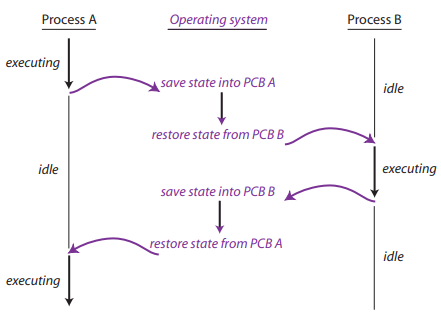
\includegraphics[scale=0.7]{context_switching}
	\end{center}
\end{solution}

\question[7]What is the real-world map-colouring problem? Explain how we might abstract this problem as a graph colouring problem. What is a planar graph? Explain how planar graphs and maps are related. Is every graph a planar graph?
\begin{solution}[2in]
	\begin{itemize}
		\item Given a plane map of regions, each contained within a continuous border, can you colour the regions of the map with 3 colours so that if any two regions touch they must be coloured differently?
		\item This can be abstracted into a graph, as all the important information is just if two regions touch
		\item \textbf{Planar Graph} - A graph that can be drawn in a plane without any graph edges crossing
		\item Every map can be turned into a planar graph
		\item Not every graph is a planar graph, some will have edges that cross
	\end{itemize}
\end{solution}

\question[2]Give a precise definition of a decision problem.
\begin{solution}[2in]
	A decision problem D consists of:
	\begin{itemize}
		\item a set of instances I
		\item A subset $Y\subseteq I$ of yes instances
	\end{itemize}
\end{solution}
\question[20]What is a graph? What is a proper colouring of a graph and an optimal
colouring of a graph? Describe two different algorithms (in English)
that enable you to colour graphs. Explain whether or not your
algorithms yield an optimal colouring (you may use graphs to illustrate
your answer if you wish). Show how your algorithms proceed when you
wish to decide whether the graph in Fig. 1 can be coloured using 4
colours
\begin{center}
	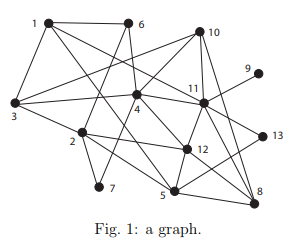
\includegraphics[scale=0.7]{graph}
\end{center}
\begin{solution}[2in]
	A graph, G=(V,E), has a finite set V of vertices and a set E of pairs of
	distinct vertices where no edge is repeated and (in an undirected
	graph) (u,v)=(v,u). A proper colouring is a colouring in which any two
	adjacent vertices are coloured differently, the optimal colouring is a
	proper colouring that uses the smallest number of colours.\\
	\\
	Algorithm one: work through the nodes in increasing order and
	colour using the smallest available colour. This will always yield a
	proper colouring, but may not yield an optimal colouring, however if
	it does yield an optimal colouring, that colouring is correct.\\
	\\
	Algorithm two: chose a node that can be coloured using the lowest
	colour possible, if there are multiple nodes that can be coloured with
	that colour, then chose the node with the lowest vertex order. Once no
	other nodes can be coloured using that colour, move onto the next
	colour.\\
	\\
	Both algorithms produce an identical 3-colouring for the graph.\\
	\\
	1:1, 2:1,3:2,4:1,5:2,6:2,7:2,8:1,9:1,10:3,11:2,12:3,13:1
\end{solution}

\question[2]Give a (not necessarily precise) definition of what it means for an algorithm to be greedy.
\begin{solution}[2in]
	An algorithm that works through a list "greedily" choosing the best thing to do
\end{solution}

\question[5]Give a precise definition of a search problem and of a solution of a
search problem.
\begin{solution}[2in]
	A search problem S consists of:
	\begin{itemize}
		\item A set of instances I
		\item A set of solutions J
		\item A binary search relation $R\subseteq I\times J$
	\end{itemize}
	In order to solve a search problem, for any instance $x\in I$ we need to:
	\begin{itemize}
		\item find a solution $y\in J$ such that $(x,y)\in R$ if there is one, or
		\item Answer no if there is no solution $y$ for which $(x,y)\in R$
	\end{itemize}
\end{solution}

\question[5]Give a precise definition of an optimisation problem and of a solution
of an instance of an optimisation problem.
\begin{solution}[2in]
	An optimisation problem O is defined as follows:
	\begin{itemize}
		\item It consists of a set of instances I
		\item for every instance $x\in I$ there is a set of feasible solutions f(x)
		\item For every instance $x\in I$ and for every feasible solution $y\in f(x)$ there is a value $v(x,y)\in \mathbb{N}=\{0,1,2,...\}$ giving the measure of the feasible solution y for the instance x
		\item There is a goal which is either min or max
	\end{itemize}
	To solve an optimisation problem, given $x\in I$, we need to find a feasible solution of maximum or minimum measure. It may be the case that:
	\begin{itemize}
		\item There are no feasible solutions for an instance
		\item For a maximisation problem, there are feasible solutions of increasingly large measure
	\end{itemize}
\end{solution}

\question[3]What is an independent set in a graph? What is the Independent Set
(optimisation) problem?
\begin{solution}[2in]
	\begin{itemize}
		\item An independent set is a set of vertices in a graph, no two of which are adjacent
		\item The independent set problem:
		\begin{itemize}
			\item An independent set U in a graph $G=(V,E)$ is a subset $I\subseteq V$ of verticies so that no vertex in U is joined by an edge to any other vertex of U
			\item A maximum independent set in G is an independent set of the greatest size possible
		\end{itemize}
	\end{itemize}	
\end{solution}

	\question[6]Detail, using pseudo-code, two different versions of Euclid's algorithm: a recursive one; and an iterative one
\begin{solution}[2in]
	Recursive:\\
	\begin{lstlisting}
	IF n==0:
	output m
	ELSE:
	set m=n and n=m mod n
	Euclid(m,n)
	\end{lstlisting}
	Iterative:
	\begin{lstlisting}
	WHILE n $\neq 0$:
	m=m-n
	IF n>m
	swap m and n
	output m
	\end{lstlisting}
\end{solution}

\question[10]First, give a natural language description of the algorithm Bubble-sort, and, next, give pseudo-code for your algorithm. Describe how your algorithm works on the input list of numbers 4,3,6,6,2,1
\begin{solution}[2in]
	\begin{itemize}
		\item The algorithm Bubble-sort repeatedly ‘passes’ through the input list of
		numbers, comparing and swapping adjacent numbers in the list.
		\item In a pass through the input list, consecutive pairs of numbers are compared
		in turn, and these numbers are swapped (in their locations) if
		the first number is greater than the second.
		\item If a swap has been made in a pass through the list then another pass
		is undertaken, otherwise the algorithm halts.
	\end{itemize}
	\begin{lstlisting}
	change = true
	WHILE change == true:
	change = false
	i = 0
	WHILE i < n - 1:
	IF A[i] > A[i + 1]:
	swap A[i] and A[i + 1]
	change = true
	i = i + 1
	output A
	\end{lstlisting}
\end{solution}
\question Here is the pseudo-code for the algorithm selection-sort
\begin{lstlisting}
pass=0
WHILE pass < n-1
x=A[pass]
i=pass+1
WHILE $i\leqslant n-1$
IF A[i]<x
swap x and A[i]
i=i+1
A[pass]=x
pass=pass+1
output A
\end{lstlisting}
\begin{parts}
	\part[4]Explain how you might amend the algorithm Selection-sort so that you no longer need the variable x	
	\begin{solution}[2in]
		\begin{lstlisting}
		pass=0
		WHILE pass < n-1
		i=pass+1
		WHILE $i\leqslant n-1$
		IF A[i]<A[pass]
		swap A[i] and A[pass]
		i=i+1
		pass=pass+1
		output A
		\end{lstlisting}
	\end{solution}	
	\part[4]Explain how you might amend the algorithm Selection-sort so that you lessen the number of data swaps made
	\begin{solution}[2in]
		\begin{lstlisting}
		pass = 0
		WHILE pass < n-1
		x=pass
		i=pass+1
		WHILE i$\leqslant$ n-1:
		IF A[i]<A[x]:
		x=i
		i=i+1
		swap A[pass] and A[x]
		pass=pass+1
		output A
		\end{lstlisting}
	\end{solution}
\end{parts}	
\droptotalpoints
\question[14]First, give a natural language description of the algorithm Merge-Sort, and, next,give pseudo-code for your algorithm (you need not provide pseudo-code to describe how two ordered lists are merged into an ordered list). Describe how your algorithm works on the input list of numbers 4,3,6,6,2,1
\begin{solution}[2in]
	\begin{itemize}
		\item Chop the input list into roughly two 'halves' so that both 'halves' either have the same length or their lengths differ by 1
		\item recursively sort each half' and
		\item merge the two sorted lists together
	\end{itemize}
	\begin{lstlisting}[mathescape=true]
	Merge-sort(l,r)
	if l<r
	m=$\lceil(r-l+1)/2\rceil-1$
	Merge-sort(l,m)
	Merge-sort(m+1,r)
	Merge(l,m,r)
	Mergesort(0,n-1)
	output A
	
	Merge(l, m, r)
	leftptr = l and rightptr = m + 1
	counter = l
	WHILE leftptr $\leqslant$ m and rightptr $\leqslant$ r:
	IF A[leftptr] $\leqslant$ A[rightptr]:
	B[counter] = A[leftptr]
	leftptr = leftptr + 1
	ELSE:
	B[counter] = A[rightptr]
	rightptr = rightptr + 1
	counter = counter + 1
	IF leftptr $\leqslant$ m:
	B[counter..r] = A[leftptr..m]
	ELSE:
	B[counter..r] = A[rightptr..r]
	A[l..r] := B[l..r]
	\end{lstlisting}
	On the input list given, it will be split into two sublists (4,3,6) and (6,2,1)\\
	These will then be recursively split until the digits are individual.\\
	Then the digits are merged back together, sorting them through the comparisons between the two sublists.\\
	The merging goes all the way up the recursion stack until the input list is sorted
\end{solution}

\question[2]Give two different ways in which a software bug can arise and give two different effects of a software bug
\begin{solution}[2in]
	\begin{itemize}
		\item Programming Error
		\item Secondary Program Error like a compiler
	\end{itemize}
\end{solution}

\question[5]Give the different aspects of the software engineering software design process known as the Waterfall model and very briefly explain what they are
\begin{solution}[2in]
	\begin{itemize}
		\item Requirements Phase - Produce a specification of what a program is supposed to do
		\item Design Phase - Compose a plan for the solution involving algorithms, data structures etc
		\item Implementation phase - Write the code
		\item Verification Phase - Test and Debug
		\item Maintenance - Continual modification/updating
	\end{itemize}
\end{solution}

\question[2]When it comes to establishing program correctness, briefly compare and contrast the different approaches taken in software testing and in formal methods
\begin{solution}[2in]
	\textbf{Formal Methods} - Mathematically based techniques for the formal specification and verification of software and hardware systems\\
	\textbf{Software Testing} - Evaluating an attribute or capability of a program or system and determine that it meets its required results
\end{solution}

\question[2]What is the difference between an algorithm being totally correct and being partially correct?
\begin{solution}[2in]
	\textbf{Totally Correct} - Correct with respect to some specification and terminates on every input\\
	\textbf{Partially Correct} - Only correct with respect to the specification 
\end{solution}

\question[4]Outline how the mathematical principle of induction and the algorithmic construction of recursion are often related in the realm of program correctness
\begin{solution}[2in]
	Induction has 3 steps:
	\begin{itemize}
		\item Formulate a property P(n)
		\item Decide upon a base case
		\item The inductive step of proving for k+1
	\end{itemize}
	With recursion we have a base case and a recursive call\\
	It is often easier to inductively prove a recursive algorithm as the base case and recursive call mirrors the inductive step
\end{solution}

\question[7]Consider the following algorithm where the input is a positive integer supplied by the variable n:
\begin{lstlisting}
algorithm: f(n):
(x,y)=(1,n)
while y!= 0:
x=x*(n-y+1)
y=y-1
output x
\end{lstlisting}
What does this algorithm do? Prove that it is totally correct
\begin{solution}[2in]
	This algorithm iteratively computes factorials.\\
	By observation, the variable y decreases by 1 at the end of every iteration of the while loop. So there will be exactly n iterations of the while loop; consequently, our algorithm always terminates.\\
	\\
	For correctness. We can also see that at the end of each iteration of the while loop, the value of n-y+1 increases by 1. Prior to the first execution of the while-loop, the value of n-y+1 is 1. Thus, by observation, during the ith iteration of the while loop, x is multiplied by i, having been initialized at 1. Consequently, after the nth iteration of the while-loop, x has the value n!. 
\end{solution}
\question[2]Give two different resources used by an algorithm that we might measure?
\begin{solution}[2in]
	\begin{itemize}
		\item Time
		\item Memory
	\end{itemize}
\end{solution}

\question[2]Why do we usually measure the time taken by an algorithm rather than
the time taken by an implementation of an algorithm?
\begin{solution}[2in]
	\begin{itemize}
		\item Not affected by language
		\item Not affected by hardware
	\end{itemize}
\end{solution}

\question[2]In pseudo-code we assume that any ‘basic’ instruction takes c units of
time to execute. What is this constant c supposed to reflect?
\begin{solution}[2in]
	The time to do one operation on a given processor
\end{solution}

\question[4]What is the worst-case time complexity of an algorithm? Why is it
expressed as a function on the natural numbers? 
\begin{solution}[2in]
	\begin{itemize}
		\item Can't give a fixed number as a bigger input will always take more time
		\item The greatest amount of time that an algorithm will take for an input
		\item How the function reacts as the input increases
	\end{itemize}
\end{solution}

\question[2]Define precisely what we mean when we say that two functions $f(n):\mathbb{N}\rightarrow\mathbb{N}$ and $g(n):\mathbb{N}\rightarrow\mathbb{N}$ are such that $f=\mathcal{O}(g)$
\begin{solution}[2in]
	There exists $n_0\in \mathbb{N}$ and $k\in Q$ such that $f(n)\leqslant k\cdot g(n)$ wherever $n\geqslant n_0$
\end{solution}

Define precisely what we mean when we say that two functions $f(n):\mathbb{N}\rightarrow\mathbb{N}$ and $g(n):\mathbb{N}\rightarrow\mathbb{N}$ are such that $f=\Omega(g)$ What does it mean in practice if we say that any algorithm solving the sorting problem has time complexity $\Omega(n\log n)$?
\begin{solution}[2in]
	If there exists $n_0\in \mathbb{N}$ and $k\in Q$ such that $f(n)\geqslant k\cdot g(n)$ wherever $n\geqslant n_0$. The algorithm takes at least $n\log n$ steps
\end{solution}

\question[5]The algorithm Bubble-sort is as follows:
\begin{lstlisting}
change = true
WHILE change == true:
change = false
i = 0
WHILE i < n - 1:
IF A[i] > A[i + 1]:
swap the numbers in A[i] and A[i + 1]
change = true
i = i + 1
output A
\end{lstlisting}
What is the time complexity of bubble-sort? (you should explain your answer)
\begin{solution}[2in]
	\begin{itemize}
		\item The inner while loop will loop n-1 times
		\item The outer loop will loop n-1 times before no swaps happen
		\item $\mathcal{O}((n-1)n+n)=\mathcal{O}(n^2)$
		\item Best case $\Omega(n)$
	\end{itemize}
\end{solution}
\question[4]What do we mean when we say that a decision problem is tractable? What is the complexity class \textbf{P}
\begin{solution}[2in]
	Tractable - It can be solved by an algorithm of time complexity $\mathcal{O}(n^k)$; that is, polynomial time\\
	\textbf{P} - The complexity class of efficiently solvable problems 
\end{solution}

\question[4]Give two objections to the definition of a tractable problem as a problem solvable in $\mathcal{O}(n^k)$ time
\begin{solution}[2in]
	\begin{itemize}
		\item What about the hidden constant
		\item What if the k is massive
	\end{itemize}
\end{solution}

\question[3]What do we mean when we say that a decision problem is efficiently checkable?
\begin{solution}[2in]
	Given a potential witness that some instance is a yes-instance, we can check in polynomial time whether the witness is indeed a witness
\end{solution}
\question[2]What is the complexity class \textbf{NP}
\begin{solution}[2in]
	The complexity class of decision problems that are efficiently checkable
\end{solution}

\question[4]Define precisely the notion of a polynomial-time transformation
\begin{solution}[2in]
	A polynomial time transformation from X to Y is an algorithm $\alpha$ that:
	\begin{itemize}
		\item Takes an instance I of X as input and provides an instance $\alpha(I)$ of Y as output
		\item Is such that an instance I of X is a yes-instance iff the instance $\alpha(I)$ of Y is a yes-instance
	\end{itemize}
\end{solution}

\question[6]Define what it means for a problem to be NP-complete. Prove that if Y is an NP-complete problem then \textbf{P=NP} if, and only if, $Y\in P$
\begin{solution}[2in]
	Suppose there is a problem $Y\in NP$ such that for any problem $X\in NP$, we have $X\rightarrow_{poly} Y$\\
	Such problems are NP complete.\\
	From the previous theorem
	\begin{itemize}
		\item If $Y\in NP$ then every problem $X\in NP$ is also in P; that is P=NP
		\item Conversely, suppose that P=NP, so, as $Y\in NP$, we must have that $Y\in P$
	\end{itemize}
	
\end{solution}


\question[2]What is Cook's theorem?
\begin{solution}[2in]
	P=NP iff $SAT\in P$
\end{solution}


\end{questions}




\end{document}